\documentclass[a4paper,10pt, twocolumn]{article}

\usepackage{float}
\usepackage{graphicx}
\usepackage{caption}
\usepackage{subcaption}
\graphicspath{{../../results/}}

\begin{document}
\section{Are EnTrI results biased?}
As transposon insertion biases can affect the essentiallity level inferred from transposon mutagenesis experiments, the dataset has been tested for two type of biases: the distance from the origin and GC content. As Figure~\ref{fig:distance_bias} shows, the insertion index decreases with the increase of the distance from the origin. Therefore, there is a bias towards the distance from the origin. However, the threshold that has been selected for essential genes (0.2) separates the two groups well.
\begin{figure}[H]
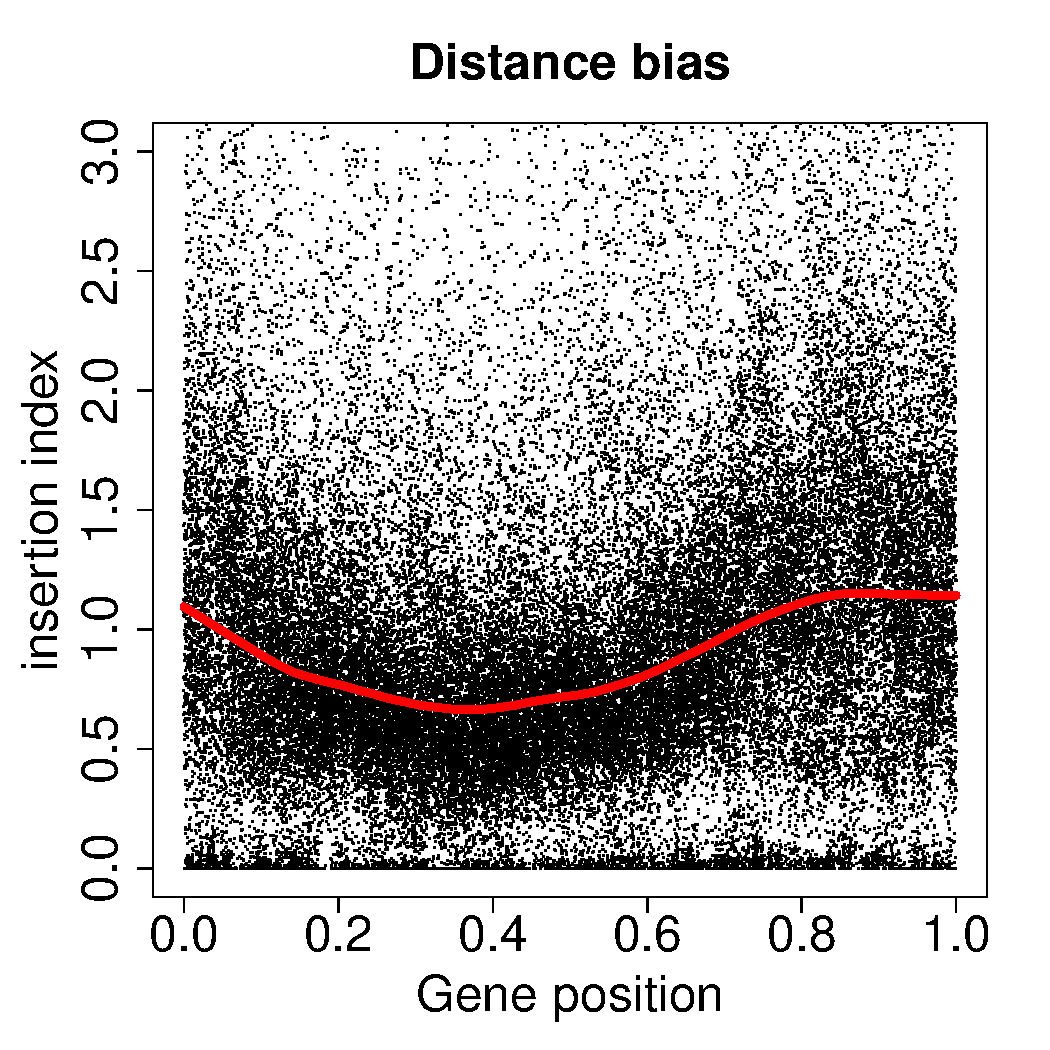
\includegraphics[scale=0.3, page=1]{biases.pdf}
\caption{The insertion index value depends on the distance from the origin}
\label{fig:distance_bias}
\end{figure}

As depicted in Figure~\ref{fig:GC_bias} there is no bias towards the GC content of the genes and the regression line is straight. The nucleotides around the insertion sites (the insertion site and 10 nucleotides on each side) are stacked on top of each other and a sequence logo is generated from these sequences to see if there is any positional bias for any nucleotide. It can be inferred from Figure~\ref{fig:logo} that there is no bias in any position except a negligible bias in the insertion site towards GC pairs. 
\begin{figure}[H]
\includegraphics[scale=0.3, page=2]{biases.pdf}
\caption{The insertion index value is not biased to GC content}
\label{fig:GC_bias}
\end{figure}

\begin{figure*}
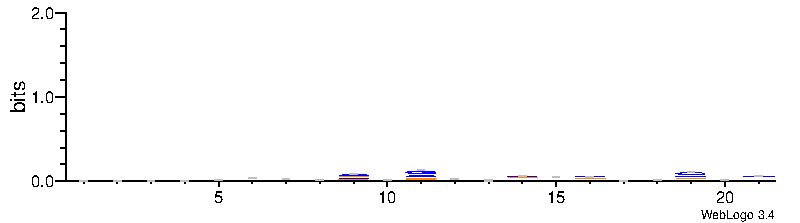
\includegraphics[scale=1.2]{logo.pdf}
\caption{There is no bias in the nucleotides around the insertion site}
\label{fig:logo}
\end{figure*}

\end{document}